\documentclass[conference]{IEEEtran}

\usepackage{mathptmx,amssymb,amsmath}
\usepackage{stmaryrd}
\usepackage{MnSymbol}
\usepackage{float}
\usepackage{amsthm}
\usepackage{array}
\usepackage[american]{babel}
\usepackage{enumerate}
\usepackage{fancyvrb}
\usepackage{cite}
%\usepackage{url}
\usepackage{mathpartir}
\usepackage{graphicx}
\usepackage{subfig}
\usepackage{color}
\usepackage{verbatim}
\usepackage{pifont}
\usepackage[lined,boxed,linesnumbered]{algorithm2e}

\widowpenalty=0
\clubpenalty=0
\displaywidowpenalty=0
\raggedbottom
\sloppy
\sloppypar

\topskip0pt
\parskip0pt
\partopsep0pt

\def\ind{\parindent}
\DefineVerbatimEnvironment{program}{Verbatim}
  {baselinestretch=1.0,xleftmargin=\ind,fontsize=\small,
   commandchars=\\\{\},samepage=true}
\DefineVerbatimEnvironment{programBox}{BVerbatim}
  {baselinestretch=1.0,xleftmargin=0pt,fontsize=\small,
   commandchars=\\\{\},samepage=true}

\def\denseitems{
    \itemsep1pt plus1pt minus1pt
    \parsep0pt plus0pt
    \parskip0pt\topsep0pt}

\def\exsep{1ex plus1ex}
\newcounter{exerc}
\newenvironment{exerc}%
{\refstepcounter{exerc}\vspace{\exsep}\noindent\hrulefill{}\nopagebreak\\%
 \noindent\textbf{Exercise \arabic{exerc}.}\ }
{\nopagebreak\par\vspace{-4pt}\noindent\hrulefill{}\vspace{\exsep}}

\newenvironment{exercSP}%
{\refstepcounter{exerc}\vspace{\exsep}
 \begin{samepage}\noindent\hrulefill{}\nopagebreak\\%
 \noindent\textbf{Exercise \arabic{exerc}.}\ }
{\nopagebreak\par\vspace{-4pt}\noindent\hrulefill{}
 \end{samepage}\vspace{\exsep}}


\def\defmacro#1{\expandafter\def\csname#1\endcsname}

\def\newdef#1#2{\expandafter\ifx\csname#1\endcsname\relax
    \defmacro{#1}{#2}%
    \else\message{Command "#1" already defined}\fi}

\newif\ifmore
\def\mapdef#1#2(#3){\def\args{#1:#2:#3,\end}%
    \moretrue
    \loop\expandafter\nextarg\args
         \ifmore\repeat}
\def\nextarg#1:#2:#3,#4\end{\def\next{#4}%
    \ifx\next\empty\morefalse
        \else\def\args{#1:#2:#4\end}\fi
    \newdef{#2#3}{#1{#3}}}

%%%
%%% Meta notes
%%%
\newcommand{\getRef}[1]{[\textbf{** #1}: \textit{refs?}]}
\newlength{\dummylen}
\newcommand{\NOTE}[1]{\setlength{\dummylen}{\fboxrule}\setlength{\fboxrule}{2pt}%
            \vspace{1ex}\noindent\hfill%
            \fbox{\begin{minipage}{.96\columnwidth}#1\end{minipage}}%
            \setlength{\fboxrule}{\dummylen}\hfill{}\vspace{1ex}}

\definecolor{red}{RGB}{255,0,0}
\definecolor{green}{RGB}{0,255,0}
\definecolor{purple}{RGB}{255,0,255}

\DefineVerbatimEnvironment{code}{Verbatim}{fontsize=\footnotesize,fontseries=b}


%%%
%%% MATH
%%%
\def\OB#1{\ifmmode#1\else\mbox{$#1$}\fi}
\newtheorem{theorem}{Theorem}
\newtheorem{lemma}{Lemma}
\newtheorem{corollary}{Corollary}
\newenvironment{definition}[1][Definition]{\begin{trivlist}
\item[\hskip \labelsep {\bfseries #1}]}{\end{trivlist}}


% shared CC definitions
% \newcommand{\OR}{\ |\ }
\newenvironment{fsyntax}{\hfill$\begin{array}{rcl@{\quad}l}}
                        {\end{array}$\hfill{\ }}
\newenvironment{syntax}{\[\begin{array}{rcl@{\quad}l}}
                       {\end{array}\]\ignorespacesafterend}
% \newenvironment{example}{\[\begin{array}{l}}
%                        {\end{array}\]\ignorespacesafterend}
\newenvironment{example}{\par\medskip\indent$\begin{array}{l}}
                       {\end{array}$\par\medskip\noindent\ignorespacesafterend}

%% overlay macros
%
\newlength{\overlaywidth}
\newlength{\overlayheight}

\newcommand{\voverlay}[3][-]{%
   \settowidth{\overlaywidth}{\mbox{\OB{#2}}}\divide\overlaywidth2%
   \hspace*{\overlaywidth}%
   \makebox[0mm]{\OB{#2}}%
   \if#1-\makebox[0mm]{\OB{#3}}\else%
         \raisebox{#1}[0mm][0mm]{\makebox[0mm]{\OB{#3}}}\fi%
   \hspace*{\overlaywidth}}

\newcommand{\vhoverlay}[3][-]{%
   \settowidth{\overlaywidth}{\mbox{\OB{#2}}}\divide\overlaywidth2%
   \settoheight{\overlayheight}{\mbox{\OB{#3}}}%
   \if#1-\else\addtolength{\overlayheight}{-#1}\fi
   \hspace*{\overlaywidth}%
   \makebox[0mm]{\OB{#2}}%
   \raisebox{-\overlayheight}[0mm][0mm]{\makebox[0mm]{\OB{#3}}}%
   \hspace*{\overlaywidth}}


%%
%% Math definitions
%%
\newtheorem{theorem}{Theorem}
\newtheorem{lemma}{Lemma}
\newtheorem{corollary}{Corollary}
\newenvironment{definition}[1][Definition]{\begin{trivlist}
\item[\hskip \labelsep {\bfseries #1}]}{\end{trivlist}}

%%% 
%%% MATH
%%%
\def\OB#1{\ifmmode#1\else\mbox{$#1$}\fi}
\newcommand{\vij}[3]{\OB{#1_{#2},\ldots,#1_{#3}}}
\newcommand{\vi}[2]{\vij{#1}{1}{#2}}
\newcommand{\vn}[2][n]{\vi{#2}{#1}}
\newcommand{\vnButi}[3][n]{\OB{#2_1,\ldots,#2_{#3-1},#2_{#3+1},\ldots,#2_{#1}}}
\newcommand{\set}[1]{\OB{\{#1\}}}
\newcommand{\vect}[1]{\OB{\langle#1\rangle}}
\newcommand{\cseq}[2][n]{\OB{^{#2:1..#1}}}
\newcommand{\iPat}[2][i]{\OB{[#1\mathop:#2]}}

% \newcommand{\xn}[1][n]{\OB{^{\bar{#1}}}}
% \newcommand{\xn}[1][n]{\OB{_{\bar{#1}}}}

\newcommand{\dom}[1]{\OB{\textit{dom}(#1)}}
\newcommand{\rng}[1]{\OB{\textit{rng}(#1)}}

\newcommand{\semL}{\OB{[\![}}
\newcommand{\semR}{\OB{]\!]}}
\newcommand{\sem}[2][{}]{\OB{\semL#2\semR_{#1}}}
\newcommand{\subst}[3]{\OB{[#1/#2]#3}}
%% multi-line definitions
\newcommand{\Begindef}{\ =\ \BegindefNES}
\newcommand{\BegindefNES}{\left\{\begin{array}{@{}l@{\quad}l}}
\newcommand{\Enddef}{\end{array}\right.}
% \newcommand{\If}{\textrm{if\ }}
\newcommand{\Otherwise}{\textrm{otherwise}}

\newcommand{\FV}[1]{\OB{\textit{FV}(#1)}}
\newcommand{\FD}[1]{\OB{\textit{FD}(#1)}}

% \newcommand{\bigstep}[3][\Delta]{\OB{#1 :- #2\Downarrow#3}}

\newcommand{\mrk}[1]{\underline{#1}}

%% 
%%  Choice calculus syntax
%%

%%% Documents and trees
% \newcommand{\prog}[1]{\texttt{#1}}
% \newcommand{\sub}[1]{\OB{{\scriptstyle\langle}#1{\scriptstyle\rangle}}}
\newcommand{\sub}[1]{\OB{\mathord\Yleft#1\mathord\Yright}}
\newcommand{\tr}[2][a]{\OB{#1\sub{#2}}}
\newcommand{\trn}[2][a]{\OB{#1\sub{\vn{#2}}}}
% \newcommand{\trPat}[4][a]{\tr[#1]{#2_{#3}|#4}}

%%% Key words & formatting/indenting
\newcommand{\CCkeyw}[1]{\textbf{\textrm{#1}}}
\newcommand{\LET}{\CCkeyw{let}}
\newcommand{\DIM}{\CCkeyw{dim}}
\newcommand{\IN}{\CCkeyw{in}}
\newcommand{\Ind}[2][{}]{\hphantom{#1}\makebox[0mm][r]{#2}\ }

%%% Choices
\newcommand{\chcL}{\langle}
\newcommand{\chcR}{\rangle}
\newcommand{\chc}[2][D]{\OB{#1\chcL#2\chcR}}
% \newcommand{\chcPP}[3][D]{\chc[#1]{\prog{#2},\prog{#3}}}

%%% Dimensions
\newcommand{\Dim}[2][D]{\OB{\DIM\ \chc[#1]{#2}}}
\newcommand{\DimIn}[3][D]{\Dim[#1]{#2}\ \IN\ #3}

%%% Let expressions
% \newcommand{\Let}[2]{\OB{\LET\ #1 = #2}\ }
% \newcommand{\Let}[3][-]{\OB{\if#1-\LET\ \else\Ind[\LET]{#1}\fi#2 = #3}}
% \newcommand{\Let}[3][\LET]{\OB{\Ind[#1]{\LET}#2 \texttt{=} #3}}
\newcommand{\Let}[3][\LET]{\OB{\Ind[#1]{\LET}#2 {\small=} #3}}
\newcommand{\LetIn}[3]{\Let{#1}{#2}\ \IN\ #3}


%%% OLD Choice notation / abbreviation
% \newcommand{\ptch}[2][L]{\OB{#2^{#1}}}
% \newcommand{\ptch}[2][L]{\OB{\overline{#2}^{#1}}}
% \newcommand{\ptch}[2][L]{\OB{#1\mathord:\ #2}}
% \newcommand{\ptch}[2][L]{\OB{#1\mathord|\ #2}}
\newcommand{\ptch}[2][L]{\OB{#1\mapsto #2}}
% \newcommand{\ptch}[2][L]{\OB{#1\to #2}}
% \newcommand{\ptch}[2][L]{\OB{#1\mathord\to #2}}
\newcommand{\ochc}[1]{\OB{\set{#1}}}
\newcommand{\chcn}[3][n]{\OB{\chc{\ptch[#2_1]{#3_1},\ldots,\ptch[#2_#1]{#3_#1}}}}
\newcommand{\ochcA}[2]{\ochc{\ptch[#1]{#2}}}
\newcommand{\ochcB}[4]{\ochc{\ptch[#1]{#2},\ptch[#3]{#4}}}
\newcommand{\ochcBi}[4]{\ochc{\ptch[\textit{#1}]{#2},\ptch[\textit{#3}]{#4}}}
\newcommand{\ochcC}[6]{\ochc{\ptch[#1]{#2},\ptch[#3]{#4},\ptch[#5]{#6}}}
\newcommand{\ochcD}[8]{\ochc{\ptch[#1]{#2},\ptch[#3]{#4},\ptch[#5]{#6},\ptch[#7]{#8}}}
%%% OLD Choice binding
\newcommand{\lbnd}[2]{\OB{#1=#2}}
\newcommand{\bnd}[2]{\OB{#1\leftarrow#2}}
\newcommand{\cbnd}[2]{\bnd{#1}{\chc{#2}}}
\newcommand{\cbind}[2]{\bnd{#1}{\chc{#2}}}
\newcommand{\bind}[3]{\OB{#1:\cbind{#2}{#3}}}
\newcommand{\bindB}[5]{\OB{#1:\cbind{#2}{#3};\cbind{#4}{#5}}}
\newcommand{\bindk}[3]{\OB{#1:\cbind{#2_1}{#3_1};\ldots;\cbind{#2_k}{#3_k}}}
\newcommand{\bindkC}[3]{\OB{#1:\bnd{#2_1}{#3_1};\ldots;\bnd{#2_k}{#3_k}}}
\newcommand{\noDbindkC}[2]{\OB{\bnd{#1_1}{#2_1};\ldots;\bnd{#1_k}{#2_k}}}
\newcommand{\noCode}{\OB{\bullet}}
\newcommand{\tagsName}{\textit{tags}}
\newcommand{\tags}[1]{\OB{\tagsName(#1)}}
\newcommand{\ctags}[1]{\OB{\textit{ctags}(#1)}}
\newcommand{\ddom}[1]{\OB{\textit{dom}^*(#1)}}

%% formatting choice names/ids
% \newcommand{\choice}[1]{\OB{{\cal #1}}}

%% names for change objects
% \newcommand{\chObj}{\OB{\omega}}
% \newcommand{\chObjB}{\OB{\omega'}}
% \newcommand{\chObj}{\OB{\bar{O}}}
% \newcommand{\chObjB}{\OB{\bar{O'}}}
% \newcommand{\vo}{\OB{\bar{O}}}
% \newcommand{\vo}{\OB{V}}
% \newcommand{\voB}{\OB{V'}}


%%
%% Static analysis
%%
\newcommand{\wdim}[2][\Delta]{\OB{#1\vdash#2}}

%%% Context notation
% \newcommand{\ctx}[1]{\OB{^{\sswarrow}C[#1]}}
%\newcommand{\ctx}[1]{\OB{\hat{C}[#1]}}
\newcommand{\ctx}[2][C]{\OB{#1[#2]}}


%%% Tag selection
\newcommand{\sel}[2][D.t]{\OB{#2\mathop\shortuparrow#1}}
% \newcommand{\tsel}[3][\Delta]{\OB{#2|_{#1}^{#3}}}
\newcommand{\tsel}[2][s]{\OB{\lfloor#2\rfloor_{#1}}}
% \newcommand{\tsel}[3][\Delta]{\OB{\sigma(#1,#2,#3)}}
% \newcommand{\tseltd}[2][\Delta]{\tsel[#1]{#2}{d.t}}
% \newcommand{\tselq}[2][\Delta]{\tsel[#1]{#2}{q}}

\newcommand{\dimSym}{\OB{\delta}}
\newcommand{\dims}[1]{\dimSym(#1)}
\newcommand{\dimProd}{\OB{\otimes}}
\newcommand{\dimSum}{\OB{\oplus}}
\newcommand{\dimUnit}{\textbf{1}}

\newcommand{\expSym}{\OB{\mu}}
\newcommand{\expEnv}{\OB{\rho}}
\newcommand{\expand}[2][\expEnv]{\expSym_{#1}(#2)}


\newcommand{\chcdep}[2]{\OB{#1\leftarrow#2}}

%% name of positional relationship
% \newcommand{\prel}{\OB{\Delta}}
% 
% \newcommand{\mkchc}[3][p]{\OB{#2[#1]\mathord{:}#3}}
% \newcommand{\addchc}[3][p]{\OB{#2[#1]\mathord{:}\mathord\cup#3}}
% \newcommand{\chcex}[2][p]{\OB{#2_{#1}}}

%% 
%%  Choice calculus semantics
%%

\newcommand{\tselB}[3]{\tsel[#3]{\tsel[#2]{#1}}}
\newcommand{\lft}[1]{\OB{\mathord\uparrow#1}}
\newcommand{\plain}[1]{\OB{\underline{#1}}}
\newcommand{\allsel}[2]{\OB{#1\mathord\Downarrow#2}}
% \newcommand{\lsel}[2][t_1,\ldots,t_n]{\OB{#2.\set{#1}}}

%%% Dimensions
\newcommand{\choicesSym}[1][{}]{\OB{\Gamma^{#1}}}
\newcommand{\choices}[2][{}]{\OB{\choicesSym[#1](#2)}}
\newcommand{\dimm}[1]{\dimSym(#1)}

%%% Variations
\newcommand{\variSym}{\OB{V}}
\newcommand{\vari}[1]{\OB{\variSym(#1)}}


%% 
%%  Design theory
%%
\newcommand{\equivSym}{\OB{\sim}}

\newcommand{\equalt}[3][C]{\OB{#2\equivSym_{#1}#3}}
\newcommand{\equtag}[3][C]{\OB{#2\equivSym_{#1}#3}}

% \newcommand{\dropName}{\textit{rem}}
% \newcommand{\drop}[4][C]{\OB{\dropName\textit{#2}_{#1}^{#3}(#4)}}
% \newcommand{\dropA}[3][C]{\drop{A}{#2}{#3}}
% \newcommand{\dropT}[3][C]{\drop{T}{#2}{#3}}
% \newcommand{\dropA}[3][C]{\OB{\alpha_{#1}^{#2}(#3)}}
% \newcommand{\dropA}[3][C]{\OB{\alpha_{#2}^{#1}(#3)}}


\newcommand{\dropi}[4][C]{\OB{\bar{#2}_{#1/#3}(#4)}}
\newcommand{\drop}[3][C]{\OB{\bar{#2}_{#1}(#3)}}

\newcommand{\dropA}[3][C]{\dropi[#1]{\alpha}{#2}{#3}}
\newcommand{\dropT}[3][C]{\dropi[#1]{\tau}{#2}{#3}}
\newcommand{\dropC}[2][C]{\drop[#1]{\gamma}{#2}}
\newcommand{\dropD}[2][C]{\drop[#1]{\delta}{#2}}



\newcommand{\vequiv}[2]{\OB{#1\sim#2}}
\newcommand{\tequiv}[4][e]{\OB{#3\equivSym^{#1}_{#2}#4}}
\newcommand{\tsubst}[4][D]{\OB{[#1:#2/#3]#4}}




%%% Properties of dimensions
% \newcommand{\indep}[2]{\OB{#1\rightleftarrows#2}}
% \newcommand{\depnd}[2]{\OB{#1\Leftarrow#2}}
\newcommand{\indep}[2]{\OB{#1\mathop\|#2}}
\newcommand{\related}[2]{\OB{#1\mathop\sim#2}}
\newcommand{\relclSym}{\OB{\vhoverlay[1.6ex]{\sim}{\scriptstyle *}}}
% \newcommand{\relclSym}{\OB{\overset{*}{\sim}}}
\newcommand{\relcl}[2]{\OB{#1\,\relclSym\,#2}}
\newcommand{\depnd}[2]{\OB{#1\rightarrow#2}}
\newcommand{\synch}[2]{\OB{#1\leftrightarrow#2}}
\newcommand{\ovlap}[2]{\OB{#1\leftrightharpoons#2}}


%%% Operations on versioned objects
\newcommand{\factorSym}{\OB{\varphi}}
\newcommand{\factor}[1]{\OB{\factorSym(#1)}}
\newcommand{\distrSym}{\OB{\delta}}
\newcommand{\distr}[1]{\OB{\distrSym(#1)}}


%%% Java example
% \newcommand{\etc}{\OB{\cdots}}
% \newcommand{\etc}{}
\newcommand{\tok}[1]{\texttt{\small #1}}
\newcommand{\toktr}[2]{\tr[\tok{#1}]{#2}}
\newcommand{\Nesting}[2]{\begin{array}[b]{@{}l@{}}%
     \tok{#1}\langle\\ \indnt#2\end{array}}
\newcommand{\End}{\rangle}
\newcommand{\indnt}{\hspace*{1em}}

\newcommand{\showEx}[1]{\medskip\noindent\centerline{#1}\medskip\noindent}

\newcommand{\class}[1]{\toktr{class}{#1}}
% \newcommand{\classNest}[1]{\Nesting{class}{#1}}
\newcommand{\List}{\tok{List}}
\newcommand{\Listg}{\tok{List<Job>}}
\newcommand{\voidName}{void}
\newcommand{\void}[1]{\toktr{\voidName}{#1}}
\newcommand{\intt}{\tok{int}}
\newcommand{\Iter}{\tok{Iter}}
\newcommand{\while}[1]{\toktr{while}{#1}}
\newcommand{\forr}[1]{\toktr{for}{#1}}
\newcommand{\Job}{\tok{Job}}
\newcommand{\run}{\tok{j.run}}
\newcommand{\ifff}{\tok{if}}
\newcommand{\nocode}{\OB{\bullet}}

% alternative content-based naming
\renewcommand{\voidName}{runJob}
\renewcommand{\intt}{\tok{trialCount}}
\renewcommand{\ifff}{\tok{break}}

\newcommand{\prel}{\OB{{\cal R}}}

% class, List/List<Job>, runJobs, trialCount, Iter, for/while, Job, j.run, break





\newcommand{\set}[1]{\ensuremath{\{#1\}}}
\newcommand{\dom}{\textit{dom}}
\newcommand{\rng}{\textit{rng}}
\newcommand{\eset}{\ensuremath{\varnothing}}
\newcommand{\OR}{\ |\ }
\newcommand{\BB}{\ensuremath{\mathbb{B}}}
\newcommand{\TT}{\ensuremath{true}}
\newcommand{\FF}{\ensuremath{false}}

% General language structure
%
\newcommand{\prog}[1]{{\small\texttt{#1}}}
\newcommand{\bs}{\texttt{\symbol{92}}}

\newcommand{\lblFmt}[1]{\textrm{\textit{#1}}}
\newcommand{\chcPP}[3][D]{\chc[#1]{\prog{#2},\prog{#3}}}
\newcommand{\chcPPP}[4][D]{\chc[#1]{\prog{#2},\prog{#3},\prog{#4}}}

%%% Choices
\newcommand{\chcL}{\langle}
\newcommand{\chcR}{\rangle}
\newcommand{\chc}[2][D]{\OB{#1\chcL#2\chcR}}

% dimensions and tags
\newcommand{\dimA}[2][a_1,a_2]{\DimIn[A]{#1}{#2}}
\newcommand{\chcA}[1]{\chc[A]{#1}}
\newcommand{\dcA}[2][a_1,a_2]{\dimA[#1]{\chcA{#2}}}

\newcommand{\dimB}[2][b_1,b_2]{\DimIn[B]{#1}{#2}}
\newcommand{\chcB}[1]{\chc[B]{#1}}
\newcommand{\dcB}[2][b_1,b_2]{\dimB[#1]{\chcB{#2}}}

\newcommand{\map}[2][\dec]{\OB{#1\mapsto#2}}

% \newcommand{\dimset}[1][D]{\OB{\bar{#1}}}
\newcommand{\dimset}[1][D]{\OB{#1^n}}
\newcommand{\xdimSym}{\textit{dim}}
\newcommand{\xdim}[1]{\OB{\xdimSym(#1)}}
% \newcommand{\xtag}[1]{\OB{\textit{tag}(#1)}}
\newcommand{\dimsSym}{\textit{dims}}
\newcommand{\dims}[1]{\OB{\dimsSym(#1)}}
\newcommand{\dimtSym}{\textit{dim}}
\newcommand{\dimt}[1]{\OB{\dimtSym(#1)}}
% \newcommand{\tags}[2]{\OB{\textit{tags}_{#1}(#2)}}

\newcommand{\decstr}{\OB{{\cal D}}}

\newcommand{\qt}[1][\decstr]{\OB{Q_{#1}}}

\newcommand{\deprel}{\OB{R}}
\newcommand{\dep}[2]{\OB{#1\mathop\to#2}}
\newcommand{\dec}{\OB{\delta}}
\newcommand{\Dec}[1][\decstr]{\OB{\Delta_{#1}}}

% \newcommand{\tg}[2][e]{\OB{#2^{#1}}}


\newcommand{\sel}[2]{\OB{#1!#2}}
\newcommand{\indep}[2]{\OB{#1\nrightleftarrows#2}}

\newcommand{\anddSym}{\OB{\wedge}}
\newcommand{\ordSym}{\OB{\vee}}
\newcommand{\andd}[2]{\OB{#1\anddSym#2}}
\newcommand{\ord}[2]{\OB{#1\ordSym#2}}
\newcommand{\all}{\OB{\star}}

\newcommand{\splt}[2]{\OB{#1\curlywedgedownarrow#2}}
\newcommand{\fcup}{\OB{\mathrel{\vec{\cup}}}}
\newcommand{\fcap}{\OB{\mathrel{\vec{\cap}}}}
\newcommand{\fsqcup}{\OB{\mathrel{\vec{\sqcup}}}}
\newcommand{\fsqcap}{\OB{\mathrel{\vec{\sqcap}}}}

% \newcommand{\nlab}{\OB{\nu}}
% \newcommand{\elab}{\OB{\eta}}
\newcommand{\nlab}{\OB{N}}
\newcommand{\elab}{\OB{E}}
\newcommand{\tN}{\tagv{\nlab}}
\newcommand{\tE}{\tagv{\elab}}
\newcommand{\tG}{\tagv{G}}
\newcommand{\tp}{\tagv{p}}
\newcommand{\vN}{\variv{\nlab}}
\newcommand{\vE}{\variv{\elab}}
\newcommand{\vG}{\variv{G}}
% \newcommand{\vG}{\variv{G}}

\newcommand{\pth}{\textit{path}}
\newcommand{\tpth}{\tagv{\textit{path}}}

\newcommand{\strp}[1]{\OB{\lfloor#1\rfloor}}

% \newcommand{\semL}{\OB{[\![}}
% \newcommand{\semR}{\OB{]\!]}}
\newcommand{\semL}{\llbracket}
\newcommand{\semR}{\rrbracket}
\newcommand{\sem}[2][{}]{\OB{\semL#2\semR_{#1}}}
\newcommand{\xsem}[2][{}]{\OB{\semL#2\semR_{#1}}}

\newcommand{\inclSym}{\ensuremath{\sqsubseteq}}
\newcommand{\incl}[2]{\ensuremath{#1 \inclSym #2}}


\newcommand{\cons}[2]{\OB{#1\mathop:#2}}

% \newcommand{\qu}{\OB{\omega}}
% \newcommand{\qd}{\OB{\rho}}
% \newcommand{\qr}{\OB{\varphi}}
% \newcommand{\id}{\OB{\iota}}

\newcommand{\filt}[2]{\OB{\langle#1,#2\rangle}}
\newcommand{\qu}{\OB{\phi}}
\newcommand{\qd}{\OB{\alpha}}
\newcommand{\qr}{\OB{\beta}}
\newcommand{\id}{\OB{\iota}}

\newcommand{\myHeader}[1]{\textbf{#1}.}

%%
%%
\newcommand{\figscale}{0.6}
\newcommand{\varsheet}{VarSheet}
\newcommand{\EUSES}{EUSES}
\newcommand{\gds}{goal-directed selection}

\newcommand{\da}{\OB{r}}
\newcommand{\spos}{\OB{p}}
\newcommand{\f}{\OB{f}}
\newcommand{\add}{\OB{a}}
\newcommand{\gid}{\OB{id}}
\newcommand{\tg}{\OB{t}}
\newcommand{\tgs}{\OB{2^t}}
\newcommand{\F}{\OB{F}}
\newcommand{\POS}{\OB{P}}
\newcommand{\p}{\OB{p}}
\newcommand{\vsheet}{\OB{s}}
\newcommand{\VSheet}{\OB{S}}
\newcommand{\V}[1]{\OB{V~#1}}
\newcommand{\TCons}{\OB{\prog{T}}}
\newcommand{\mapname}[1]{\textit{#1}}
\newcommand{\dset}[1]{\{#1\}}
\newcommand{\gcell}[1]{\##1}
\newcommand{\ltText}{\OB{<_{r}}}
\newcommand{\eqText}{\OB{\equiv_{r}}}
\newcommand{\ltRel}[2]{#1 \ltText #2}
\newcommand{\eqRel}[2]{#1 \eqText #2}



\newcommand{\posSym}{\OB{\pi}}
\newcommand{\varSym}{\OB{V}}
\newcommand{\fmlSym}{\OB{\varphi}}
\newcommand{\pos}[1]{\posSym(#1)}
\newcommand{\var}[1]{\varSym(#1)}
\newcommand{\fml}[1]{\fmlSym(#1)}
\newcommand{\lbl}{\OB{l}}
\newcommand{\Lbl}{\OB{L}}
\newcommand{\uniset}{\OB{S}}

\newcommand{\variSym}{\OB{VS}}
\newcommand{\vari}[1]{\OB{\variSym(#1)}}


\newcommand{\htdim}{Housing\&Transportation}
\newcommand{\lpdim}{Loan Payment}

\newcommand{\A}{\OB{A}}
\newcommand{\natset}{\mathbb{N}}
\newcommand{\checked}{\text{\ding{51}}}
\newcommand{\unchecked}{\text{\ding{55}}}
\newcommand{\undecided}{\OB{\bullet}}


\pagestyle{plain}
\date{}

\begin{document}

\title{A Model for Representing Variational Spreadsheets
\thanks{This work is partially
supported by the Air Force Office of Scientific
Research under the grant FA9550-09-1-0229 and by the
National Science Foundation under the grant CCF-0917092.
}}

\author{
\IEEEauthorblockN{Martin Erwig}
\IEEEauthorblockA{Oregon State University\\
                  erwig@eecs.oregonstate.edu}
\and
\IEEEauthorblockN{Duc Le}
\IEEEauthorblockA{Oregon State University\\
                  ledu@eecs.oregonstate.edu}
\and
\IEEEauthorblockN{Eric Walkingshaw}
\IEEEauthorblockA{Oregon State University\\
                  walkiner@eecs.oregonstate.edu}
}

\maketitle

\begin{abstract}
TBD
\end{abstract}

\section{Introduction}
\label{sec:intro}

In this paper we address the problem of working with variation in
spreadsheets. Variation in software is an area of growing interest \cite{SPL,
FOSD, ...}. One reason is that the demands on modern software to adapt to
different environments is constantly increasing. The individualization of
software to the needs of a particular company, person, or even with regard to
when or where it is used is one important driving force.
%
As a software for particular application domains, spreadsheets are no
different and also face the need to be flexible and adaptable.

So far the question of variation in spreadsheets has only been touched
tangentially in research. There has been some work on computing differences
between spreadsheets \cite{CEL10hcc,Scaffidi12hcc.}, but this work has focused
on identifying variation and does not offer solutions to the problem of how to
represent, work with, and reason about variation on spreadsheets.

In this paper we propose a formal model for variational spreadsheets, analyze
some of its formal properties, and demonstrate how this model can be used as a
basis for future spreadsheet systems.
%
Specifically, we will demonstrate how we can systematize the work with
variation through the two concepts of \emph{dimension} and \emph{choice}. This
systematic approach to the representation of variation in spreadsheets allows
the identification of consistency criteria that can be exploited to develop
tools for finding errors in spreadsheets.
%
Moreover, we will illustrate how variational spreadsheets can support the
exploratory design of spreadsheets. In many situations the definition of a
spreadsheet model offers alternative ways of representing data and formulas,
and a decision of what the best way is to do that is often not clear.
Variations allow the spreadsheet designer/programmer to develop different
model variants in parallel and defer the decision to a later point.

\NOTE{Continue with an example. Make sure that each aspect of the example
points to a technical problem/issue and say where in the paper this issue will
be addressed.}


We first give a motivating example for \varsheet.
Figure~\ref{fig:before} shows a conventional spending estimate of a
college student. Suppose the student is not happy with it, they would
adjust the costs of some categories based on available options. After
some adjustments, the student ends up with the spreadsheet in
Figure~\ref{fig:after}, for which they pay \$50 less. In the updated
spreadsheet, the housing cost is \$50 less since the rented house is
further from campus, but that would increase the cost of transportation.
The student also decides to pay \$100 less on their loan. Considering
both versions, the student would probably go after the latter one, and
by doing this, they lose the chance to reduce another \$50. Had the
student chosen the original housing option and kept Loan payment to be
\$500, the monthly cost would have been \$1450.
%
Figure~\ref{fig:selection} shows a possible user interface of
\varsheet~that could support the student in their decision making
process. There are three variation points in the spreadsheet. The
\mapname{\htdim} categories are related and thus grouped into a red box
with a dashed line separating the two available options. In \varsheet,
\mapname{\htdim} is called a \emph{dimension}---a choice users have to
make. A dimension contains a set of options, each being called a
\emph{tag}. \mapname{\htdim}'s tags are \mapname{Close} and
\mapname{Far}. The \mapname{\lpdim} dimension represents a different
variation point with two tags \mapname{500} and \mapname{600} and thus
is colored differently (green). The last variation point, the
\mapname{Total} category, does not contain variational formulas by
itself. The formula being used is \prog{SUM(B2:B6)} and is
non-variational, yet the cell inherits the variational structures of its
referred cells and hence contains four available options. This cell is
therefore colored purple to indicate that it contains \emph{induced
variation}. Showing all the four alternatives of \mapname{Total} gives
the student an overview of all the different options they have.
Moreover, if the student selects the \$1450 alternative, \varsheet~will
automatically make decisions for \mapname{\htdim} and \mapname{\lpdim},
and displays those decisions and the resulting spreadsheet to them. We
call this feature \emph{\gds}, the process of selecting spreadsheet
variants based on certain goals.

\begin{figure}
\centering
    \subfloat[Before] {
        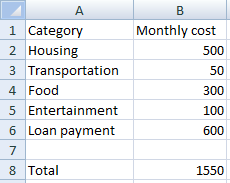
\includegraphics[scale=\figscale]{img/before}
        \label{fig:before}
    }\hspace{2em}
    \subfloat[After] {
        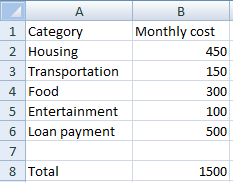
\includegraphics[scale=\figscale]{img/after}
        \label{fig:after}
    }\hspace{2em}
    \subfloat[A Possible User Interface] {
        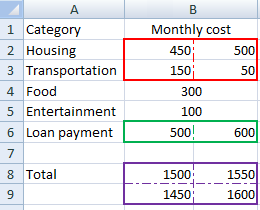
\includegraphics[scale=\figscale]{img/selection}
        \label{fig:selection}
    }
\caption{A Monthly Spending Spreadsheet}
\label{fig:mspending}
\end{figure}

The study of variational spreadsheets brings up several insights to
current research on software variation. While traditional variation
mechanisms focus on either the syntax or semantics domain, spreadsheets'
immediate semantics computation expands the application of variational
constructs to both domains, enabling the realization of \gds. In the
example above, Loan payment varies syntactically while Total varies
semanticallly, and one could even define cells that vary on both
domains.
%
Existing variational contructs mainly work on linear or tree structures,
which localizes their scope of impact. Spreadsheets have a special two
dimensional structure that makes localization hard to achieve. For
instance, in Figure~\ref{fig:before}, one could replace row 4 by the
spreadsheet in Figure~\ref{fig:food} and expects this variation
introduction to be local. This action unfortunately has a global impact
on the spreadsheet's structure and the addresses/values of several
unrelated cells. The Monthly Cost column has to be shifted to column C,
while the Total column has to be shifted one row down. In our
variational spreadsheet model, we provide mechanisms to localize the
effect of structural changes.

\begin{figure}
\centering
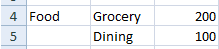
\includegraphics[scale=\figscale]{img/food}
\caption{A Different Way to Represent the Food Category}
\label{fig:food}
\end{figure}

Lastly, by letting users actively define variation in spreadsheets, we
remove the need for using spreadsheet diffing algorithm, which can be
imperfect and misleading at times.

% In following sections of the paper, we first discuss the background
% and related work in section~\ref{sec:background}. Then we % begin
% describing the syntax of \varsheet~in section \ref{sec:syntax}, which is
% followed by section \ref{sec:semantics} about the language's semantics.
% Section \ref{sec:langprops} discusses several axiomatic rules that
% could be used to transformed, % while section \ref{sec:eval} provides an
% evaluation of our language on the \EUSES~corpus \cite{Ii05theeuses}.
% Section \ref{sec:concl} concludes the paper.

\section{Background and Related Work}
\label{sec:background}

\NOTE{To be rewritten}

\NOTE{Talk about the prototype of the VLHCC 2011 paper}

Existing empirical research demonstrates the need for an effective
approach to deal with spreadsheet variation. Spreadsheet reusing is
common, but users often have to choose from various options [citation
needed]. Once a spreadsheet is chosen and several modifications have
been made to it, if users recognize that it was not the right one to
begin with, they will have to start all over again on a different one.
This could happen for many times until users are happy with their
choice. To mitigate this problem, \varsheet~ gives users the ability to
modify multiple versions/spreadsheets at the same time on a single
representation and select a desired version later. Another reason for
spreadsheet variation is due to spreadsheet errors and debugging.
Spreadsheets contain errors \cite{Panko98whatwe}\cite{Powell2008128},
many of which are introduced in the process of reusing and modifying
existing spreadsheets. When debugging, users often need to show the
differences between multiple versions, so a framework for systematically
managing changes is needed.

In the area of spreadsheet change support, existing tools can be
classified into two big categories: change tracking tools and
spreadsheet diffing tools. One representative example of a change
tracking tool is Microsoft Excel's change tracking feature, which
provides users the ability to track spreadsheet edits such as inserting
rows, updating equations, etc. This tool is useful and effective in
helping users understand versioning information of spreadsheets but is
not without limitation. The entire variational spreadsheet is
represented using only the time dimension. It is not possible to group
changes into categories or groups such that they can be undone or
applied again. Another problem arises when two or more users copy and
modify the same original spreadsheet. When trying to merge the modified
copies, it is unclear which change includes or excludes other changes.
For \varsheet, grouping changes could simply be resolved by changing
dimension/choice names, which will be defined in the next sections.
Research and commercial tools for diffing spreadsheets are prevalent,
including CC DiffEngineX \cite{DiffEngineX} and Synkronizer
\cite{Synkronizer}. These tools are effective in comparing spreadsheets
and producing accurate results. However, they do not reveal the original
purposes of users' changes and do not provide a way to document those.

On a broader topic, there has been extensive research on the topic of
representing and managing software variation. The two big pillars of
this topic is the compositional approach \cite{KA08}, which modularizes
software product line features \cite{CN01} into individual folders and
describes variability at a higher level using feature models
\cite{Bat05}, and the annotated approach \cite{KA08}, where variability
is encoded and represented inside source code. Since there are
advantages and disadvantages for each approach, Erwig and
Walkingshaw~\cite{EW11tosem} designed the Choice Calculus to shorten the
gap between them and to take advantage of the approaches' benefits. The
Choice Calculus's design is based on the idea that software variation
should be done at both source code and higher levels with
not-too-restrictive and not-too-relaxed constraints, making it highly
applicable for tree-like structures. \varsheet~expands Choice Calculus's
ideas of dimensions and choices to the spatial, two dimensional
structure of spreadsheets.

\section{Dimensions and Decisions}
\label{sec:dims}

A \emph{dimension} describes one way in which something varies.  For example,
\mapname{\htdim} in our example in Figure~\ref{fig:mspending} is one
dimension of variation.
%
A \emph{dimension definition} assigns a \emph{dimension name} to a non-empty
set of \emph{tags}, which correspond to the alternatives in that dimension.  A
dimension definition is written as $D=\set{t_1,\ldots,t_n}$,
%
for example,
% the mode of transportation dimension can be represented as
$\htdim=\set{Close, Far}$.
%
A \emph{qualified tag} is a tag prefixed by the name of the dimension it is
taken from, written $D.t_i$. Qualified tags are used to distinguish between
tags of the same name from different dimensions. Given a qualified tag $q=D.t$,
we can extract the dimension name  with the function $\xdim{q}=D$.
% and the tag with the functions $\xdim{q}=D$ and $\xtag{q}=t$.


A \emph{decision space} of \emph{degree} $n$ is given by a set of $n$
dimension definitions $\dimset = \set{D_1=T_1, \ldots, D_n=T_n}$ where $T_i$
is the set of tags for dimension $D_i$.
%
We define the function $\dims{\dimset}=\set{D_1,\ldots,D_n}$ to return the set
of all dimension names in a decision space.
% , and $\tags{\dimset}{D_i}=T_i$ to return
% the tags of dimension $D_i$ in decision space $D^n$.
%
The \emph{tag universe} of decision space $D^n$, written $\qt[n]$, is the set
of all qualified tags in $D^n$, defined as
$\qt[n]=\set{D.t\ |\ D\in\dims\dimset\wedge t\in D}$.


A \emph{decision} in a decision space \dimset\ is a set of
qualified tags $\dec\subseteq\qt[n]$ that contains at most one tag for each
dimension, that is, $q,q'\in\dec\implies q=q'\vee\xdim{q}\neq\xdim{q'}$.
%
We overload the function \dimsSym\ to also denote the dimension names of a
decisions, that is, $\dims{\dec}=\bigcup_{q\in\dec}\xdim{q}$.
% $\dims{\dec}=\bigcup_{q\in\dec}\xdim{q}$.
%
A decision $\dec\subseteq\qt[n]$ is \emph{complete} if it contains
a qualified tag from every dimension in $D^n$, that is, if
$\dims{\dec}=\dims{D^n}$, otherwise it is \emph{partial}.

\section{Variational Spreadsheets}

A variational spreadsheet represents a family of related plain
spreadsheets, each being called a \emph{variant}.
Figure~\ref{fig:before} and~\ref{fig:after} show two of the four
variants of the monthly spending spreadsheet. Each variant contains a
subset of a universe set of \emph{variational cells} $\uniset$.

Variational cells encode information about which variants the cells
belong to, where they appear in the spreadsheet grid structure, and what
types of content they store. Each variational cell has an unique address
$\add$ from the set $\A$. We define a label function
$\varSym:\A\to2^{\qt[n]}\cup\set{\unchecked}$ to label each cell with
either a decision $\dec$ or the \unchecked~symbol to
provide support for defining variational spreadsheets' semantics.
$\varSym$ helps decide whether a cell belongs to a variant. Each cell
also contains a \emph{formula} $\f\in\F$, which can be a value, an
address reference, or a function on other formulas.

\[
\begin{array}{lcl@{\qquad}l}
\f \in \F & ::= & v  & \textit{values} \\
         & \OR & \add & \textit{identity references} \\
         & \OR & \OB{\omega} (\f, \ldots, \f) & \textit{functions}\\
\end{array}
\]

\noindent
In the above definition, $\F$ represents the set of all formulas, $v$
ranges over primitive values (integers, etc.), and $\omega$ stands for
the set of all possible functions on formulas. We define a function
$\fmlSym:\A\to\F$ to map cell addresses to formulas and a function
$\posSym:\A\to\POS$ to generate \emph{spatial embeddings} given cell
addresses. Spatial embeddings $\p = (\natset, \natset)$ are stored as
pairs of natural numbers and are used to aid a pretty printing algorithm
in computing cells' concrete embeddings or positions on the
two-dimentional grid. The first number in $\p$ represents relative
vertical embeddings while the second represents horizontal embeddings.

A variational spreadsheet combines a decision space $\dimset$ and the
universe set of variational cells and is defined by the tuple $(\dimset,
\varSym, \fmlSym, \posSym)$.

In Figure~\ref{fig:idedsheet} we provide two variants of a variational
spreadsheet containing a single dimension $\mapname{D} = \set{D.1,
D.2}$. Relative embedding are shown on the top-right corner of each
cell, and cell addresses are shown on the top-left corner. The universe
set of cells contains all the cells with addresses \gcell{1--10}. We
leave the contents of several cells blank as they are not important for
our discussion. The cell at address \gcell{2}'s formula is \prog{\#5 +
1}, yet the formula is pretty printed as \prog{C1 + 1} and \prog{D1 + 1}
since cell \gcell{5}'s concrete embedding changes from one variant to
another. Two different types of cells exist in
Figure~\ref{fig:idedsheet}, \emph{non-variational} and
\emph{variational} cells. Non-variational cells are cells that appear in
all variants whereas variational cells do not. Non-variational cells'
tags are the empty set $\emptyset$, and variational cells' tags are
either partial or complete decisions $\dec$. We provide the cells' tags below.

\[
\begin{array}{l@{\ : \ }l}
    \gcell{1}, \gcell{2}, \gcell{5}, \gcell{6} & \emptyset \\
    \gcell{3}, \gcell{4} & \dset{\mapname{D.1}} \\
    \gcell{7}, \gcell{8}, \gcell{9}, \gcell{10} & \dset{\mapname{D.2}} \\
\end{array}
\]

\NOTE{Note that we can always allow tags like $\set{A.1, B.1, B.2}$ since,
due to the semantics definitions, $\set{A.1, B.1, B.2}$ is the same as $\set{A.1}$
in the case the $B$ has only two tags. If $B$ has more than two tags, $\set{A.1, B.1, B.2}$
is ``syntactic sugar'' for the two labels $\set{A.1, B.1}$ and $\set{A.1, B.2}$ }

The pretty printing algorithm places the cell with the lowest horizontal
and vertical embeddings at \prog{A1} and recursively adds cells to the
grid based on the following conventions.

\begin{itemize}
    \item Cells with the same vertical embedding are on the same column.
    Cells with the same horizontal embedding are on the same row.
    \item For all pairs of cells $x$ and $y$, if $x$'s horizontal embedding
    is less than $y$'s, $x$'s row number has to be less than $y$'s.
    \item For all pairs of cells $x$ and $y$, if $x$'s vertical embedding is
    less than $y$'s, $x$'s column number has to be less than $y$'s.
\end{itemize}

\begin{figure*} [ht]
\centering
\subfloat[Variant 1]{
    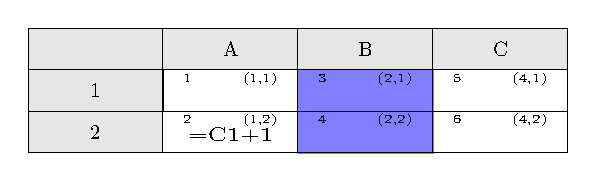
\includegraphics[scale=\figscale]{tikz/v1}
    \label{fig:v1}
}
\subfloat[Variant 2]{
    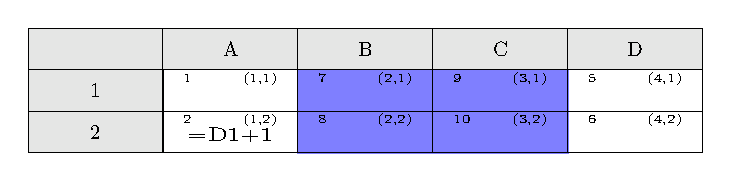
\includegraphics[scale=\figscale]{tikz/v2}
    \label{fig:v2}
}
\caption{Two variants of a variational spreadsheet}
\label{fig:idedsheet}
\end{figure*}

\section{Semantics}
\label{sec:semantics}
\newcommand{\semP}{\sem[P]}

The pretty printing algorithm works on individual variants, which are
selected by picking a subset of cells from the cell universe. A natural
question is how do we know which cells to pick. To answer this question,
in this section we describe \emph{variation semantics}, a mapping
between complete decisions and spreadsheet variants.\footnote{Note that
we ignore the discussion about the semantics of individual variants
since they are basically the semantics of plain spreadsheets.}
Each variant corresponds to a complete decisions $\dec$, and a cell $c$ belongs
to the variant if $\var{c} \subseteq \dec$. For instance, a cell whose
label is $\set{A.1}$ belongs to all the variants whose decisions are supersets
of $\set{A.1}$.

The steps involved in computing variation semantics are: (1) generating
all complete decisions, (2) performing \emph{tag selection} on those
decisions to mark several cells as excluded (\unchecked), and (3)
collect all remaining cells into variants and map corresponding
decisions to those variants. 

\subsection*{Dimensions and Complete Decisions}
\newcommand{\dimColText}{\textit{dims}}
\newcommand{\dimCol}[1]{\OB{\dimColText(#1)}}
\newcommand{\tagsText}{\textit{tags}}
\newcommand{\tagsCell}[1]{\OB{\tagsText(#1)}}
\newcommand{\decisionsText}{\textit{decisions}}
\newcommand{\decisions}[1]{\OB{\decisionsText(#1)}}
\newcommand{\examplesheet}{\OB{sh}}

The set of complete decisions of a variational spreadsheet \vsheet~is
defined below with $D^n$ being \vsheet's decision space.

\begin{align*}
\decisions{s} = \{\{D_1.t_1, \ldots, D_n.t_n\} \ |\ & \{D_1,\ldots,D_n\} = \dims{D^n}\\
        & \wedge \forall i \in \set{1\ldots n}, t_i \in D_i\}
\end{align*}

\subsection*{Tag Selection}

\newcommand{\tsel}[2][s]{\OB{{\lfloor#2\rfloor}_{#1}}}
\newcommand{\stsel}[2][s]{\OB{{\lfloor#2\rfloor}_{#1}}}
\newcommand{\compatibleSym}{\OB{\sim}}
\newcommand{\compatible}[2]{\OB{#1\compatibleSym#2}}
\newcommand{\updateText}{\textit{update}}
\newcommand{\update}[2]{\updateText(#1, #2)}
% A cell is excluded from a variant when it is marked as \unchecked.
Tag selection applies complete decisions to variational spreadsheets and
mark several cells as excluded (\unchecked). First, each cell at address
$\add$'s \emph{label} is instantiated as the cell's tags $\var{\add}$.
During the tag selection process, the cell's label either becomes
\unchecked~or get reduced to a smaller set of tags.
The set of labels is $\Lbl = 2^{\qt[n]} \cup \set{\unchecked}$.

The single tag selection operation $\stsel[]{} : \Lbl \times \qt[n]
\rightarrow \Lbl$ is defined as

\[
\begin{array}{l@{ = }ll}
    \stsel[\tg]{\unchecked} & \unchecked & \\
    \stsel[\tg]{\lbl} & \begin{cases}
                        \lbl \setminus \set{\tg} &, \textrm{if } \tg \in \lbl \\
                        \lbl                     &, \textrm{if } \tg \not\in \lbl \wedge \dim(\tg) \not\in \dims{\lbl}\\
                        \unchecked &, \textrm{otherwise} \\
                     \end{cases} \\
\end{array}
\]

We overload the complete tag selection operation $\tsel[]{} : \Lbl
\times 2^{\qt[n]} \rightarrow \Lbl$ as below.

\[
\begin{array}{l@{ = }l}
    \tsel[\emptyset]{\lbl}          & \lbl  \\
    \tsel[\set{\tg} \cup ts]{\lbl}  & \tsel[ts]{\stsel[\tg]{\lbl}} \\
\end{array}
\]

Variation semantics is thus defined as
\[
\begin{array}{r@{\ =\ }l}
    \vari{\vsheet} & \{(ts, \{c \ |\ c\in\vsheet\wedge\tsel[ts]{\var{c}} \neq \unchecked\})\
                                  |\ ts \in \decisions{\vsheet}\} \\
\end{array}
\]


\NOTE{With the semantics defined above, we can even remove the condition  $ts_1 \cap ts_2 = \emptyset$}
\begin{lemma}
If $ts_1 \cap ts_2 = \emptyset$,
\[
\tsel[ts_1 \cup ts_2]{\lbl} = \tsel[ts_2]{\tsel[ts_1]{\lbl}} = \tsel[ts_1]{\tsel[ts_2]{\lbl}}
\]
\end{lemma}

\section{Variational Choices}
\label{sec:choices}

\newcommand{\cdims}{\OB{ds}}
\newcommand{\calts}{\OB{as}}
\newcommand{\clist}[1]{\OB{[#1]}}
\newcommand{\listlen}[1]{\OB{length(#1)}}
\newcommand{\setsize}[1]{\OB{|#1|}}
\newcommand{\unionchcsym}{\OB{\uplus}}
\newcommand{\unionchc}[2]{#1\unionchcsym#2}


While each cell in a variational spreadsheet is labeled individually,
the entire spreadsheet exhibits a common pattern---several sets of cells
are alternatives of one another. For instance, in Figure~\ref{fig:idedsheet},
$\set{\gcell{3}, \gcell{4}}$ is an alternative of $\set{\gcell{7}, \gcell{8},
\gcell{9}, \gcell{10}}$. Since presenting cells and tags in a linear fashion does not
reveal this pattern, in this section we define the notion of \emph{choices} to
explicitly represent alternatives. 

A choice denotes one or more dimensions/decisions to be made and contains a 
set of alternatives, each being a pair of a decision and a set of cells. 
Formally, choices are defined as a pair (\cdims, \calts) satisfying the
following conditions.

\NOTE{I did not include the position conditions in this section since they
seem to be a bit arbitrary. We can add those later if we want to}

\[
\begin{array}{l}
\cdims \subseteq \dims{\dimset}, \cdims \neq \emptyset \\
\calts = \set{(\dec_1, s_1), \ldots, (\dec_k, s_k)}  \\
\forall i \in \set{1..k}, s_i \subseteq \uniset, \forall i \neq j, \dec_i \neq \dec_j \\
\forall i \in \set{1..k}, \forall c \in s_i, \var{c} \subseteq \dec_i\\
\setsize{\calts} = \prod_{D_i \in \cdims}{\setsize{D_i}} \\
\end{array}
\]

Each element in $\calts$ represents a complete decision with regard
to $\cdims$ and the alternative obtained by applying that decision.
The aforementioned example can be represented as the choice
\[
(\set{A}, \set{(\set{A.1}, \set{\gcell{3}, \gcell{4}}), 
(\set{A.2}, \set{\gcell{7}, \gcell{8},\gcell{9}, \gcell{10}})})
\]

To simplify this notations, from now on we assume each dimension contains two tags, 
$\forall A, A = \set{A.1, A.2}$, and we use the notation $\chcA{s_1, s_2}$ to represent 
$(\set{A}, \set{(\set{A.1}, s_1), (\set{A.2}, s_2)})$. Using the same convention, the notation 
$\chcA{\chcB{s_{11}, s_{12}}, \chcB{s_{21}, s_{22}}}$ is
equivalent to
\begin{align*}
(\set{A,B}, \set{& (\set{A.1, B.1}, s_{11}), (\set{A.1, B.2}, s_{12}),\\
                 & (\set{A.2, B.1}, s_{21}), (\set{A.2, B.2}, s_{22})}) \\
\end{align*}

Any variational spreadsheet can be partitioned into sets of choices and non-variational cells.
In the following spreadsheet, every cell is represented by a tuple of three elements: address,
label, and position. The set of five cells can be split into two choices 
$\chcA{\set{\gcell{1}}, \set{\gcell{2}}}$ and $\chcA{\chcB{\set{\gcell{3}}, \emptyset}, 
\chcB{\emptyset, \gcell{4}}}$ and a set $\set{\gcell{5}}$.

\[
\begin{array}{l}
    (\gcell{1}, \set{A.1},(1,1)) \\
    (\gcell{2}, \set{A.2},(1,1)) \\
    (\gcell{3}, \set{A.1, B.1},(2,1)) \\
    (\gcell{4}, \set{A.2, B.2},(2,1)) \\
    (\gcell{5}, \emptyset,(3,1)) \\
\end{array}
\]

\NOTE{We can talk about the algorithm to derive the set of choices here, but it's really simple}

This enables us to look at variational spreadsheet from a different angle where choices 
and sets of non-variational cells are combined into variational spreadsheets. 
We define the $\unionchcsym$ operator to combine choices
and sets. The above spreadsheet can be represented as

\[
\unionchc{\unionchc{\chcA{\set{\gcell{1}}, \set{\gcell{2}}}}{\chcA{\chcB{\set{\gcell{3}}, \emptyset},
\chcB{\emptyset, \gcell{4}}}}}{\set{\gcell{5}}}
\]
\noindent
$\unionchcsym$ is commutative, associative and performs similarly to set union when being applied to
two sets. 

Given this \emph{choice-directed} representation of spreadsheets, we can define an alternative way to 
compute spreadsheet semantics. For every complete decision $\dec$, each choice in the choice-directed
representation is resolved to an alternative that is simply a set. For example, given the decision 
$\set{A.1, B.1}, \chcA{\set{\gcell{1}}, \set{\gcell{2}}}$ is resolved to $\set{\gcell{1}}$, while
\chcA{\chcB{\set{\gcell{3}}, \emptyset},\chcB{\emptyset, \gcell{4}}} is resolved to $\set{\gcell{3}}$.
We can then compute the union of those alternatives and the set of non-variational cells to form 
the corresponding variant for the decision $\dec$.

\NOTE{We formalize this semantics if we want. This should be pretty easy as well}

We can now talk about several properties of choices and variants. The transformations below
are semantics-preserving. Note that all the conditions for choices mentioned above have to be satisfied.
\[
    \chcA{s,s} = s
\]
This transformation is also true when \chcA{s,s} is an alternative of a different choice $B$.

\[
    \unionchc{s_1}{\chcA{a_1,a_2}} = \chcA{\unionchc{s_1}{a_1}, \unionchc{s_2}{a_2}}
\]

In this equation, $a_1$ and $a_2$ can either be sets of cells or choices.

\[
    \unionchc{\chcA{a_1, a_2}}{\chcB{a_3,a_4}} 
                    = \begin{cases}
                          \chcA{\unionchc{a_1}{a_3}, \unionchc{a_2}{a_4}}, \text{ if } A == B\\
                          \chcA{\chcB{\unionchc{a_1}{a_3}, \unionchc{a_1}{a_4}},
                                \chcB{\unionchc{a_2}{a_3}, \unionchc{a_2}{a_4}}}, \text{ otherwise }\\
                      \end{cases} \\
\]


% \section{Language Properties}
% \label{sec:langprops}



% \begin{proof}
% ...
% \end{proof}



% \NOTE{TODO: Add three more theorems: (1) C-S equivalent (choice expansion), (2) Reduction of tags, (3) Dimension dependency theorem}

% \NOTE{Some laws are: (1) Orders does not matter when performing tag selection.
% (2) What about the composition of two variational spreadsheets?
% (3) What does the addressing scheme affect the representation?
% }

\section{Conclusion and Future Work}
\label{sec:concl}
TBD

\bibliographystyle{abbrv}
\bibliography{change,me}

\end{document} 